\documentclass{standalone}

\usepackage{tikz}
\usetikzlibrary{arrows.meta, decorations.markings}

\tikzset{
    midarrow/.style={
        decoration={markings, mark=at position 0.53 with {\arrow{Latex}}},
        postaction={decorate}
    }
}

\begin{document}
	
	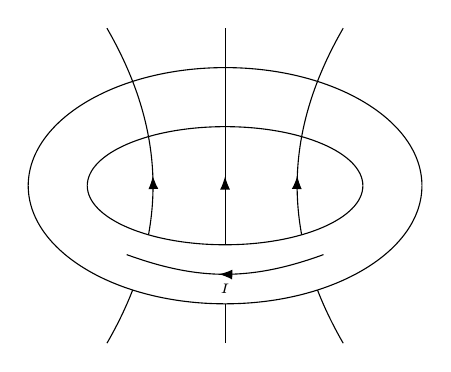
\begin{tikzpicture}
	
	\def\Rx{2.5}
	\def\rx{1.75}
	\def\Ry{1.5}
	\def\ry{0.75}
	
		% Moitié haute du tore
		\draw (-\rx,0) [x radius=\rx cm, y radius=\ry cm] 
    arc[start angle=180, end angle=0]; 
    	\draw (\Rx,0) [x radius=\Rx cm, y radius=\Ry cm] 
    arc[start angle=0, end angle=180];
    	
    	% flèches de champ
    	\def\anglediff{30}
    	\def\sepx{1.5}
    	\draw[midarrow]
  			(-\sepx, -2)
    		to [out=90-\anglediff, in=-90+\anglediff]
    		(-\sepx,2);
		\draw[midarrow]
  			(0, -2)
    		to [out=90, in=-90]
    		(0,2);
    	\draw[midarrow]
  			(\sepx, -2)
    		to [out=90+\anglediff, in=-90-\anglediff]
    		(\sepx,2);
    		
    	
    	% On efface les lignes qui doivent se trouver derrière la partie avant du tore
    	\fill[white] (-\rx,0) [x radius=\rx cm, y radius=\ry cm] 
    arc[start angle=180, end angle=360] -- 
    	(\Rx,0) [x radius=\Rx cm, y radius=\Ry cm] 
    arc[start angle=360, end angle=180] -- cycle;
    
    	% Moitié basse du tore
		\draw (-\rx,0) [x radius=\rx cm, y radius=\ry cm] 
    arc[start angle=180, end angle=360]; 
    	\draw (\Rx,0) [x radius=\Rx cm, y radius=\Ry cm] 
    arc[start angle=360, end angle=180];
    
    % Flèche du courant toroïdal
    	
    	\draw[midarrow]
  			(\Rx/2, -\Ry/3-\ry/2)
    		to [out=200, in=-20]
    		(-\Rx/2, -\Ry/3-\ry/2);
    	\node[anchor=north] at (0, -\Ry/2-\ry/2) {\tiny \( I \)};    		
	
	\end{tikzpicture}
\end{document}